%%%%%%%%%%%%%%%%%%%%%%%%%%%%%%%%%%%%%%%%%%%%%%%%%%%%%%%
\documentclass{article}
%%%%%%%%%%%%%%%%%%%%%%%%%%%%%%%%%%%%%%%%%%%%%%%%%%%%%%%
\usepackage[utf8]{vietnam}
%%%%%%%%%%%%%%%%%%%%%%%%%%%%%%%%%%%%%%%%%%%%%%%%%%%%%%%
\usepackage{graphicx}
%%%%%%%%%%%%%%%%%%%%%%%%%%%%%%%%%%%%%%%%%%%%%%%%%%%%%%%
\usepackage{hyperref}
%%%%%%%%%%%%%%%%%%%%%%%%%%%%%%%%%%%%%%%%%%%%%%%%%%%%%%%
\usepackage{xcolor}
\pagecolor[RGB]{40, 42, 54} % Đặt màu nền
\color[RGB]{18, 161, 24} % Đặt màu chữ
%%%%%%%%%%%%%%%%%%%%%%%%%%%%%%%%%%%%%%%%%%%%%%%%%%%%%%%
\usepackage{float} % Cố định hình ảnh [H]
%%%%%%%%%%%%%%%%%%%%%%%%%%%%%%%%%%%%%%%%%%%%%%%%%%%%%%%
\begin{document}
%%%%%%%%%%%%%%%%%%%%%%%%%%%%%%%%%%%%%%%%%%%%%%%%%%%%%%%
\tableofcontents
\newpage
%%%%%%%%%%%%%%%%%%%%%%%%%%%%%%%%%%%%%%%%%%%%%%%%%%%%%%%
\listoffigures
\newpage
%%%%%%%%%%%%%%%%%%%%%%%%%%%%%%%%%%%%%%%%%%%%%%%%%%%%%%%
\section{Tuần 3: Xây dựng dashboard}
%%%%%%%%%%%%%%%%%%%%%%%%%%%%%%%%%%%%%%%%%%%%%%%%%%%%%%%
\subsection{Bài 1}

\subsubsection{Thực hành tạo dashboard theo video}

\begin{figure}[H]
\centering
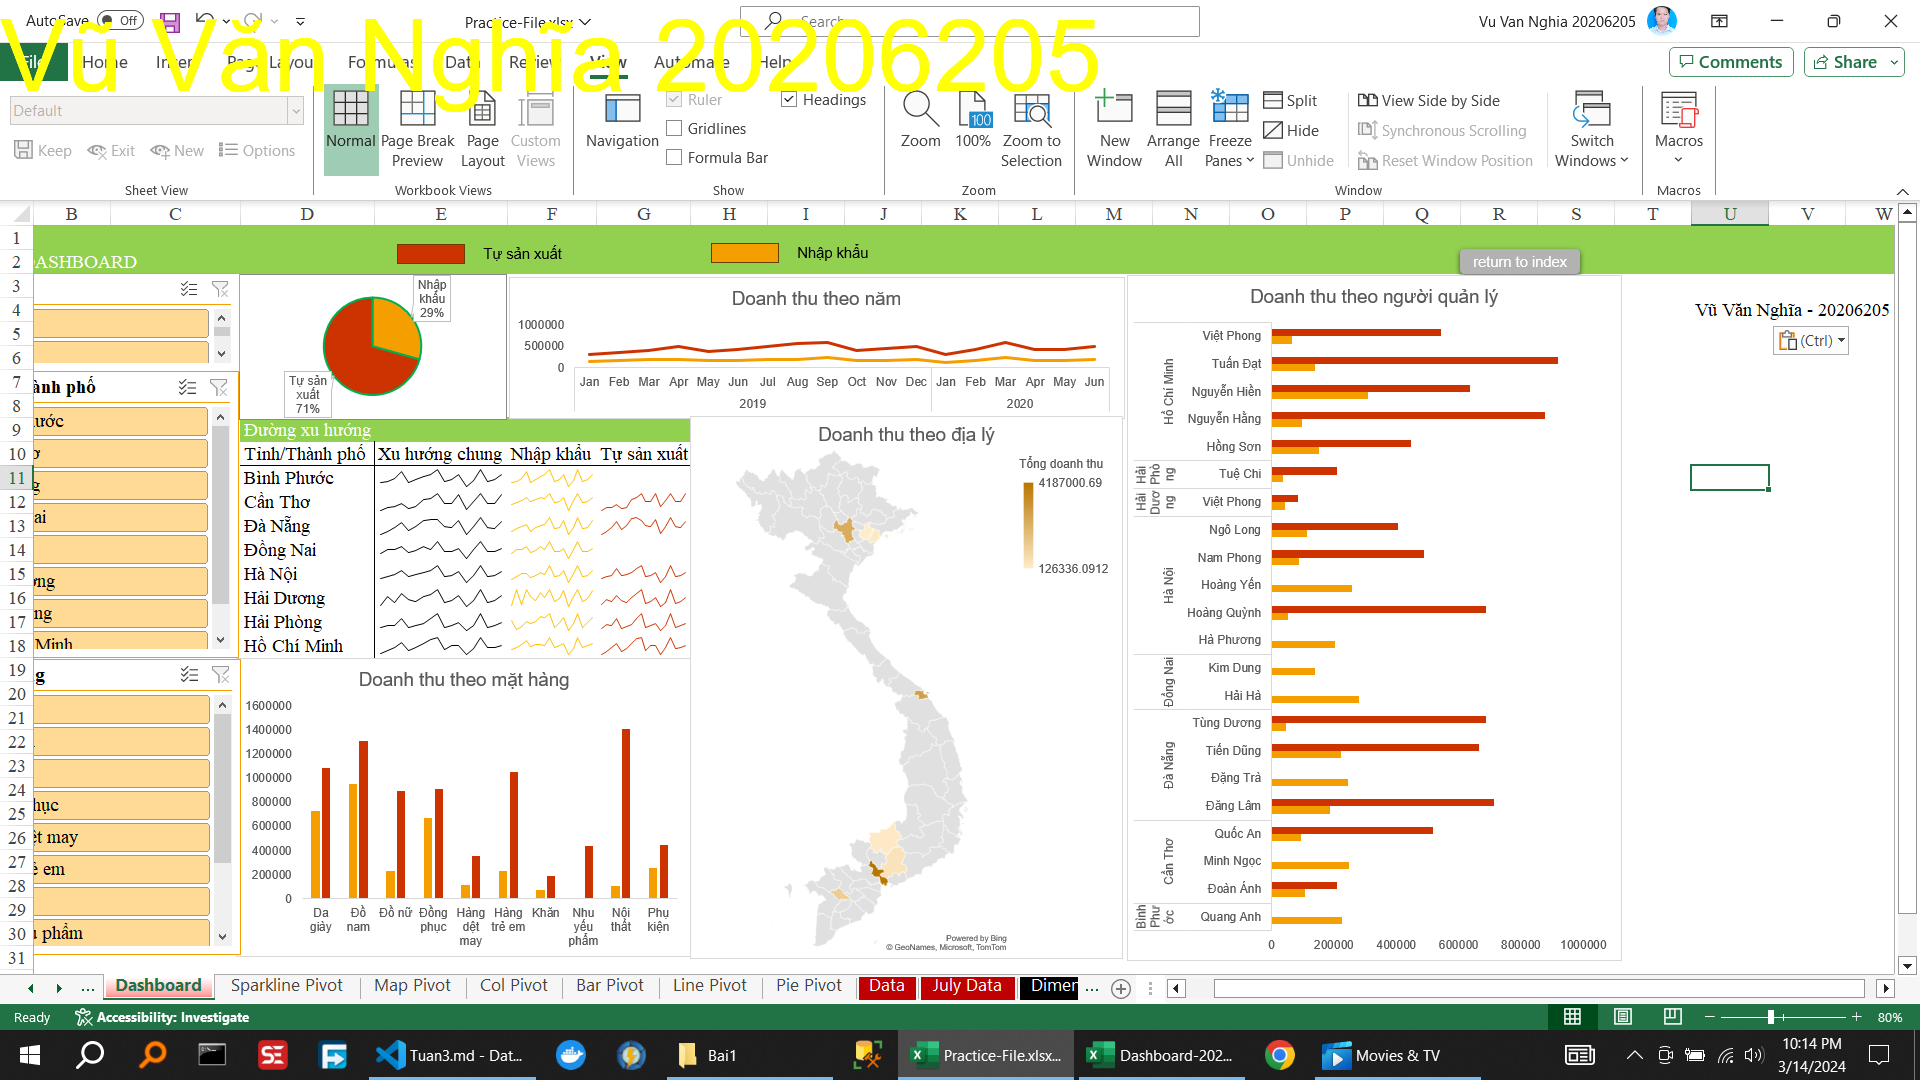
\includegraphics[scale = 0.15]{Bai1/ThucHanh/0.png}
\caption{Thực hành tạo dashboard theo video}
\end{figure}

\subsubsection{Thực hành phân tích dashboard}

\begin{itemize}
\item Đọc dashboard và phân tích
\begin{itemize}
\item Dashboard dùng để mô tả về doanh số bán hàng cho thị trường Việt Nam.
\item Dashboard có các biểu đồ:
\begin{itemize}
\item Biểu đồ tròn: thể hiện tỷ lệ nhập khẩu và tự sản xuất.
\item Biểu đồ đường: thể hiện doanh thu theo năm.
\item Biểu đồ thanh: thể hiện doanh thu theo người quản lý.
\item Biểu đồ cột: thể hiện doanh thu theo mặt hàng.
\item Biểu đồ bản đồ: thể hiện doanh thu theo địa lý.
\end{itemize}
\end{itemize}
\item Xác định các chiều (DIM), các các yếu tố phân tích (FACT)

\begin{figure}[H]
\centering
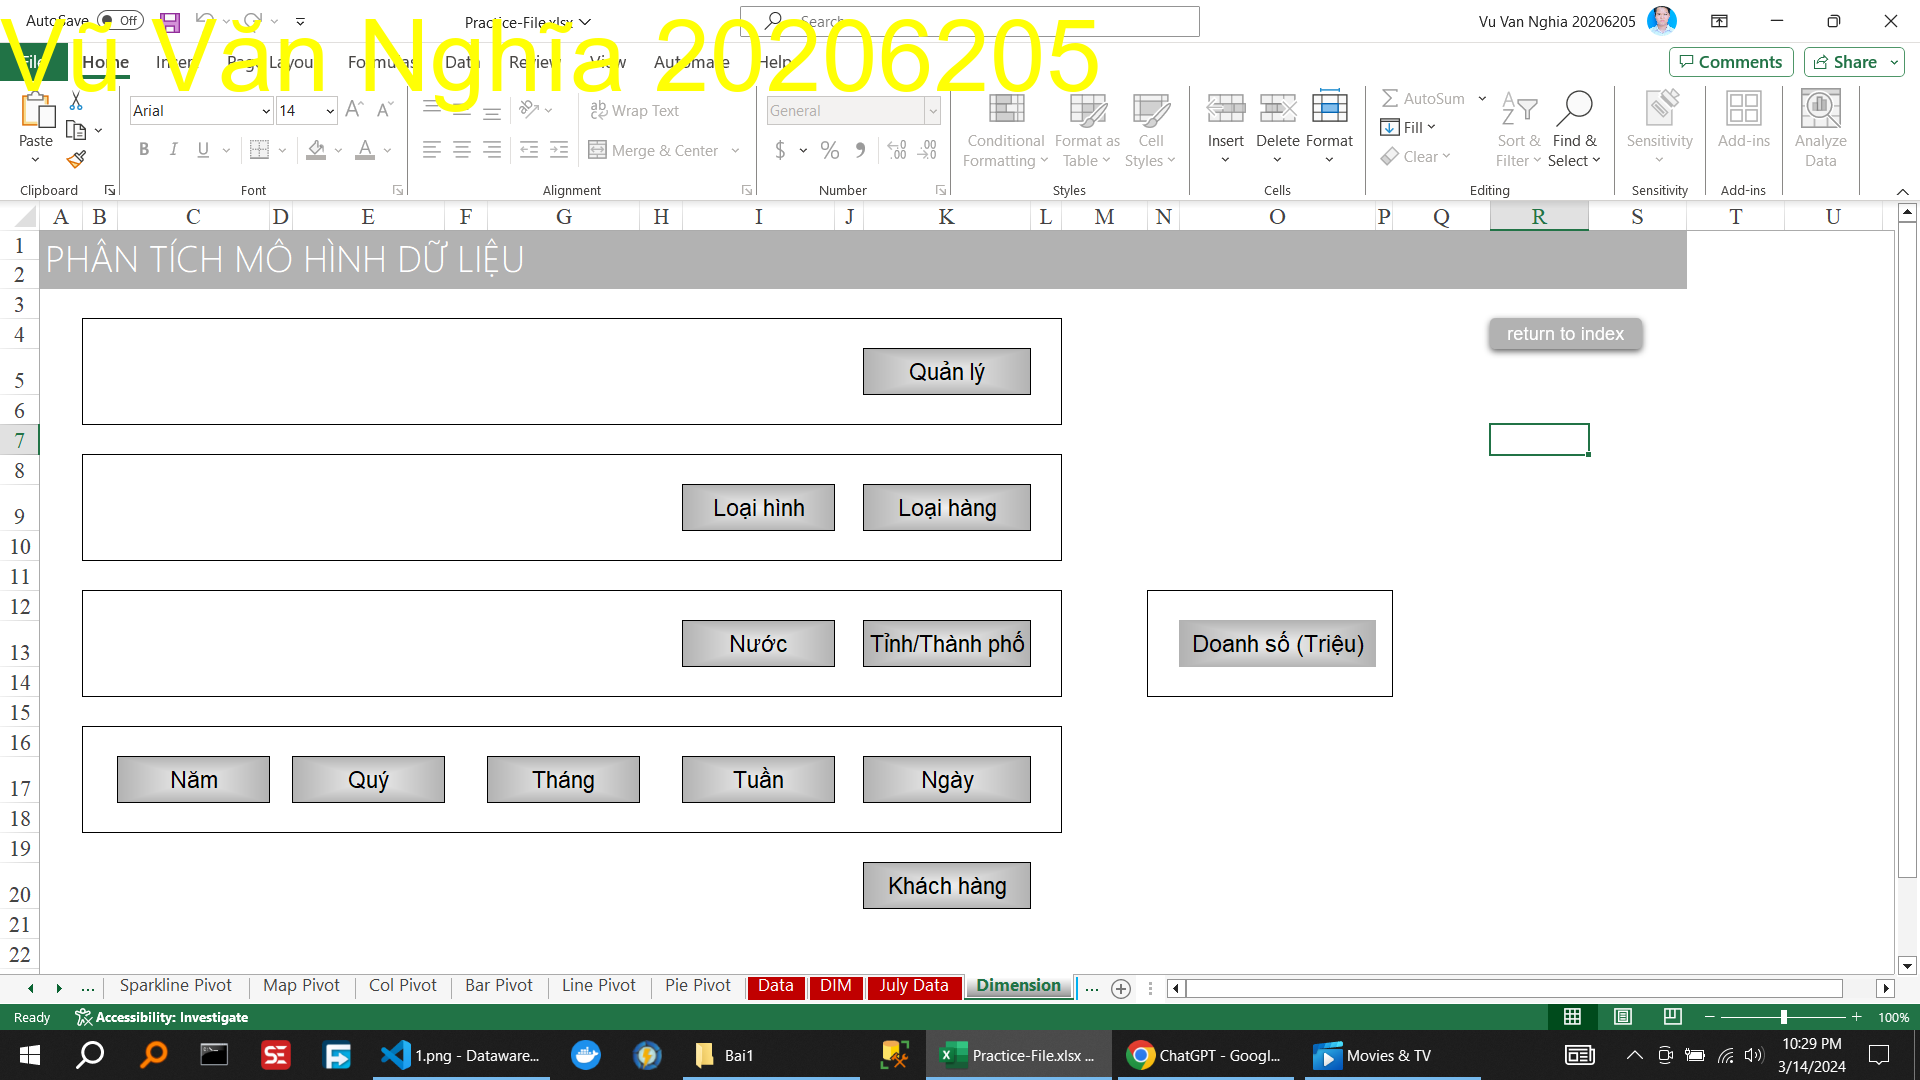
\includegraphics[scale = 0.15]{Bai1/ThucHanh/1.png}
\caption{Thực hành xác định các chiều (DIM), các các yếu tố phân tích (FACT)}
\end{figure}

\begin{itemize}
\item DIM: Thời gian, Năm, Loại hình Sản xuất, Tỉnh/Thành phố, Nước, Quản lý, Mặt hàng, Khách hàng.
\item FACT: Doanh số (Triệu).
\end{itemize}

\item Sử dụng công cụ Remove Duplicate để tạo ra con voi khái niệm các chiều.

\begin{figure}[H]
\centering
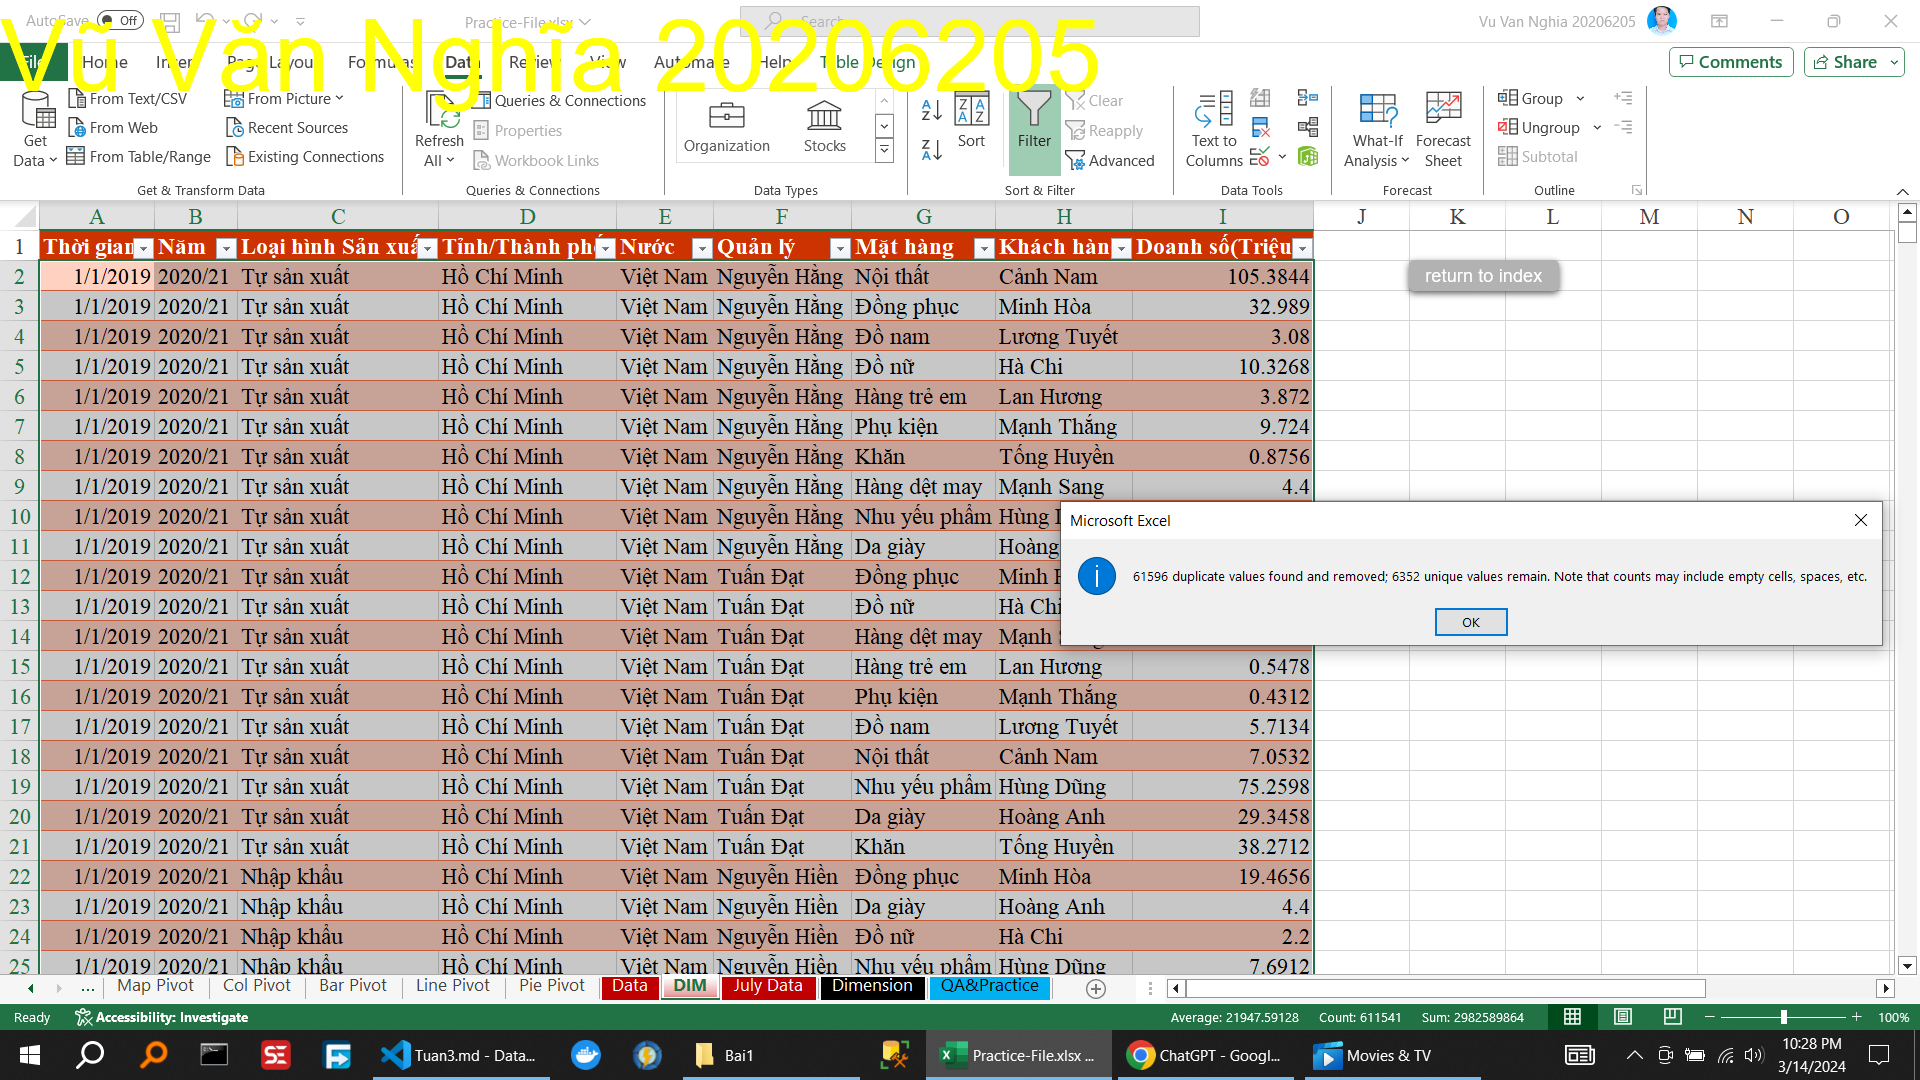
\includegraphics[scale = 0.15]{Bai1/ThucHanh/2.png}
\caption{Thực hành sử dụng công cụ Remove Duplicate để tạo ra con voi khái niệm các chiều}
\end{figure}

\end{itemize}

%%%%%%%%%%%%%%%%%%%%%%%%%%%%%%%%%%%%%%%%%%%%%%%%%%%%%%%
\subsection{Bài 2}

% % @ \subsubsection{Thực hành tạo dashboard}

% % \begin{figure}[H]
% % \centering
% % @ 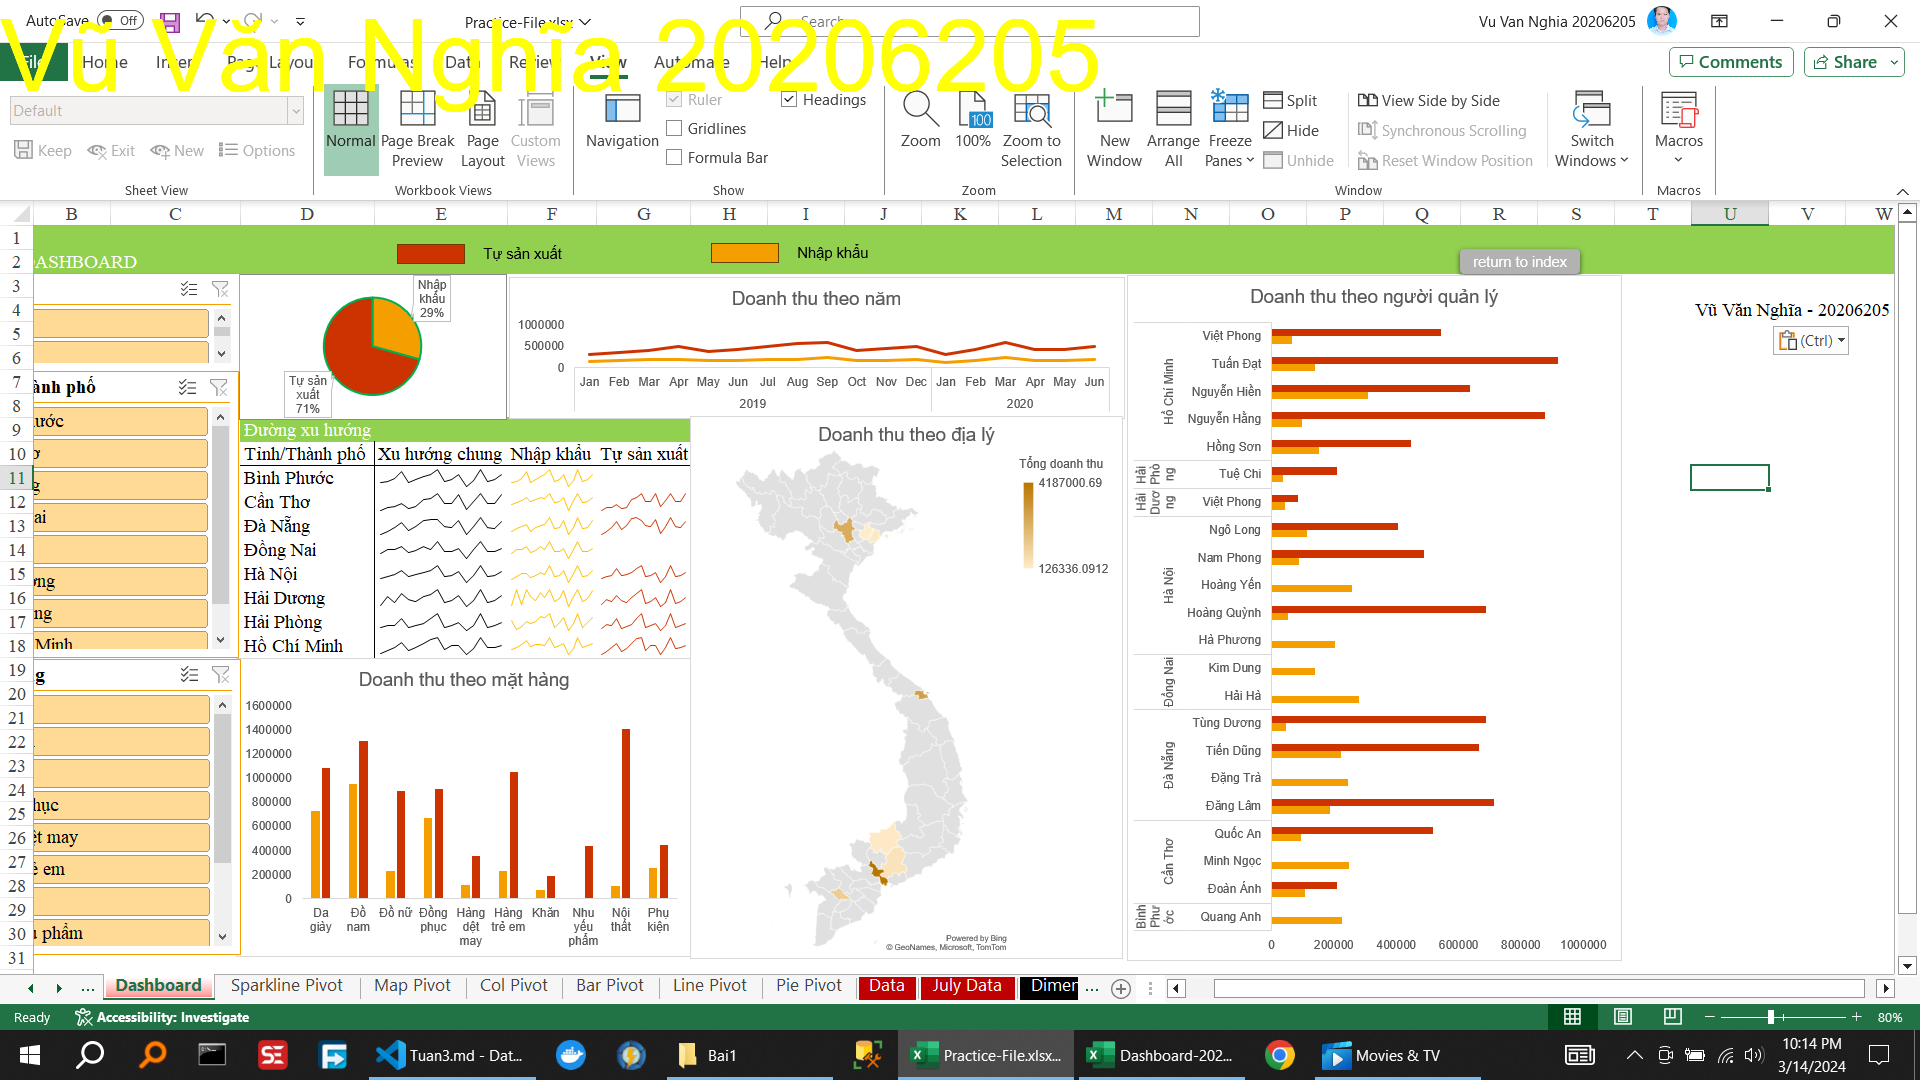
\includegraphics[scale = 0.15]{Bai1/ThucHanh/0.png}
% % \caption{Thực hành tạo dashboard}
% % \end{figure}

% \subsubsection{Thực hành phân tích dashboard}
% % Viết Requirement cần phân tích
% Chúng tôi cần ccccc
% Để viết các yêu cầu phân tích cho tập tin Excel có các tiêu đề như trên, bạn cần xác định mục tiêu cụ thể của việc phân tích dữ liệu. Dưới đây là một số yêu cầu phân tích mẫu dựa trên thông tin đã cung cấp:

% 1. **Yêu cầu tổng quan:**
% - Phân tích dữ liệu đơn hàng để hiểu về hoạt động kinh doanh của công ty.
% - Tìm hiểu về xu hướng bán hàng, doanh số, và hiệu suất bán hàng theo thời gian, sản phẩm, v.v.

% 2. **Phân tích về đơn hàng:**
% - Xác định số lượng đơn hàng được đặt hàng (QUANTITYORDERED) và giá trị đơn hàng (SALES).
% - Phân tích xu hướng đặt hàng theo thời gian (ORDERDATE).
% - Phân tích tình trạng đơn hàng (STATUS) để hiểu về tình hình xử lý đơn hàng.

% 3. **Phân tích về sản phẩm:**
% - Đánh giá hiệu suất bán hàng của các dòng sản phẩm (PRODUCTLINE) dựa trên doanh số và số lượng đặt hàng.
% - So sánh giá bán thực tế (PRICEEACH) với giá đề xuất (MSRP) để đánh giá chính sách giá và chiến lược giá cả.

% 4. **Phân tích về khách hàng:**
% - Phân tích khách hàng dựa trên thông tin như tên khách hàng (CUSTOMERNAME), số điện thoại (PHONE), và địa chỉ (ADDRESS).
% - Đánh giá doanh số bán hàng của từng khách hàng và tìm hiểu về mối quan hệ với khách hàng.

% 5. **Phân tích về địa lý:**
% - Phân tích phân phối địa lý của khách hàng (CITY, STATE, COUNTRY) để hiểu về thị trường tiềm năng và mối quan hệ địa lý.

% 6. **Phân tích về thời gian:**
% - Phân tích doanh số bán hàng theo quý (QTR_ID), tháng (MONTH_ID), và năm (YEAR_ID) để nhận biết xu hướng theo mùa và các thay đổi theo thời gian.

% 7. **Phân tích về kích thước giao dịch:**
% - Phân tích kích thước giao dịch (DEALSIZE) để hiểu về phân phối các giao dịch theo kích thước và phân loại giao dịch.

% 8. **Phân tích về sales và marketing:**
% - Đánh giá hiệu suất của các chiến dịch marketing dựa trên doanh số bán hàng và số lượng đơn hàng.

% 9. **Phân tích về quốc gia và khu vực:**
% - So sánh hiệu suất bán hàng giữa các quốc gia và khu vực (COUNTRY, TERRITORY) để xác định các thị trường tiềm năng và mối quan hệ kinh doanh.

% 10. **Phân tích về thông tin liên lạc:**
% - Phân tích thông tin liên lạc của khách hàng (CONTACTLASTNAME, CONTACTFIRSTNAME) để hiểu về mối quan hệ với khách hàng và quản lý danh sách liên lạc.

% Mỗi yêu cầu phân tích này có thể được mở rộng và tùy chỉnh phù hợp với mục tiêu kinh doanh cụ thể của bạn.

% % Xác định các DIM, FACT
% hình ....
% text ....

% % Vẽ voi DIM
% hình ....

% % Xây dựng một dashboard trên dữ liệu này theo requirement
% vẽ excel ....

% % Phân tích trên dashboard vừa xây dựng
% .....

%%%%%%%%%%%%%%%%%%%%%%%%%%%%%%%%%%%%%%%%%%%%%%%%%%%%%%%
\end{document}
%%%%%%%%%%%%%%%%%%%%%%%%%%%%%%%%%%%%%%%%%%%%%%%%%%%%%%%